\documentclass{beamer}

\usepackage{fontspec}
\usepackage{xeCJK}
\setCJKmainfont{DFFN_R3.TTC}
\XeTeXlinebreaklocale "zh"
\XeTeXlinebreakskip = 0pt plus 1pt
\linespread{1.3}
\allowdisplaybreaks

\newcommand{\weib}{\CJKfamily{weib}}
\newcommand{\hkss}{\CJKfamily{hkss}}
\newcommand{\hksy}{\CJKfamily{hksy}}
\newcommand{\lth}{\CJKfamily{lth}}
\usepackage{color}
\usepackage{booktabs}
\usepackage{tabularx}
\usepackage{caption}
\usepackage{tikz}
\usepackage{verbatim}
\usepackage{pgfplotstable}
\pgfplotsset{width=12cm}
\pgfplotsset{height=7cm}
\pgfplotsset{compat=1.13}

\usetheme{EastLansing}
\usetikzlibrary{positioning}
\useinnertheme{rectangles}
\usefonttheme{professionalfonts}

\newcommand{\lw}{0.8mm}
\setbeamercovered{transparent}


%\AtBeginSection[]
%{
  %\begin{frame}<beamer>
	%\frametitle{報告大綱}
	%%\frametitle{RoadMap}
    %\tableofcontents[currentsection]
  %\end{frame}
%}

\title{Paper Introduction}
\subtitle{\textcolor[rgb]{0.00,0.50,1.00}{{Speech Processing \& Machine Learning Laboratory}}}
\author{徐瑞陽}
\date{2019/03/20}
\begin{document}



\begin{frame}
\maketitle
\end{frame}

\begin{frame}
\frametitle{Outline}
\tableofcontents
\end{frame}

\section{Interesting Facts about Adversarial Attack/Defense}
\subsection{Background Knowledge}
\begin{frame}{Amount of Information Adversary had}
    \begin{itemize}
      \item White-Box: Adversary has \textbf{full-access} to the model (structure, weight)
      \item Black-Box: Labels assigned by the \textbf{Oracle} for chosen input (e.g API call)
    \end{itemize}
\end{frame}

\begin{frame}{Optimization View on Adversarial Robustness}
  \begin{block}{Objective}
    \[ \min_\theta \mathbb{E}_{(x,y) \sim \mathcal{D}}[\max_{\delta \sim \mathcal{S}}L(x+\delta,y|\theta)]\]
  \end{block}
  \begin{itemize}
    \item $\mathcal{S}$: allowed pertubations of adversary
    \item $\theta$: weights of classifier model
  \end{itemize}
\end{frame}

\begin{frame}{Allowed Pertubations of Adversary}
  \begin{itemize}
    \item Distance metric
      \begin{itemize}
        \item $L_0$: \# of pixel can change
        \item $L_2$: move within Euclidean ball with radius $\epsilon$
        \item $L_\infty$: every pixel has $\epsilon$ budget to move around
      \end{itemize}
  \end{itemize}
\end{frame}

\begin{frame}{Optimization Methods of Adversary}
  How to find the most adversarial point within $\mathcal{S}$?
  \begin{itemize}
    \item Gradient (First Order Adversary), the most common one
    \item Mixed Integer Programming \\
      $\rightarrow$ \href{https://openreview.net/forum?id=HyGIdiRqtm}{Evaluating Robustness of Neural Networks with Mixed Integer Programming, ICLR2019}
      
    \item And more...
  \end{itemize}
\end{frame}
\begin{frame}{One Adversary Instance - FGSM}
  \textit{Fast Gradient Sign Method} is an \color{blue}{$L_\infty\text{-bounded}$}  \color{purple}{first-order} \color{black}{adversary}
  \[
    \tilde{x} = x + \epsilon \, \texttt{sgn} \nabla_xL(x,y|\theta)
  \]

  Some variants as follows
  \begin{itemize}
    \item multi-step (possibly w/ projection)
    \item ensemble
  \end{itemize}
\end{frame}

\subsection{Obfuscated Gradients Give a False Sense of Security}
\begin{frame}{Obfuscated Gradients Give a False Sense of Security}
  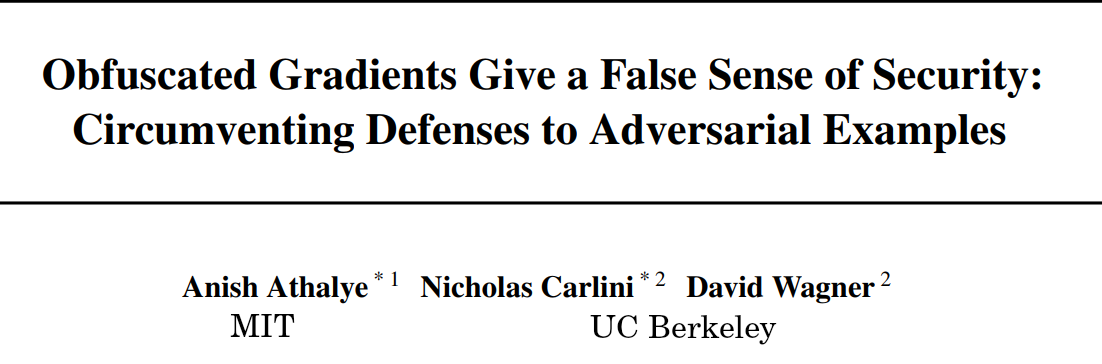
\includegraphics[width=\textwidth]{fig/ob-grad/ob-grad-title.png}
  \center ICML 2018
\end{frame}

\begin{frame}{Some Highlights}
  \begin{itemize}
    \item Provide a method to identify so-called \textbf{Obfuscated Gradients}
    \item Identify 7/9 of defenses proposed in ICLR 2018 succeed defensing by this pheonemon
    \item \textbf{Provide simple algorithms to beat those defenses} \href{https://github.com/anishathalye/obfuscated-gradients}{$\rightarrow$ github}\\
      (within pertubations $\mathcal{S}$ they claim they can defend under white-box setting)
  \end{itemize}
\end{frame}

\begin{frame}{It's Da Lian Time}
  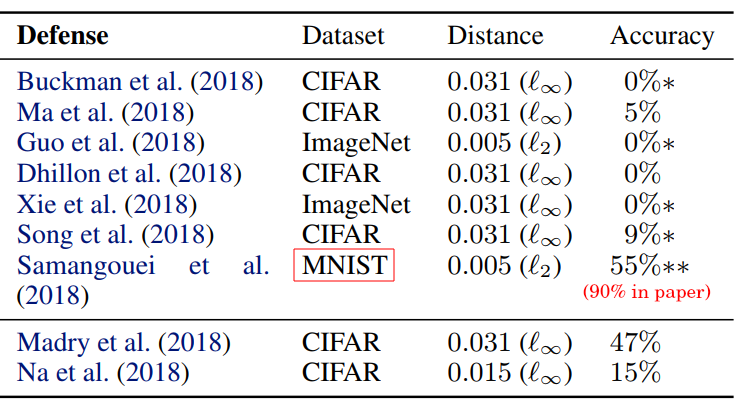
\includegraphics[width=\textwidth]{fig/ob-grad/table.png}
\end{frame}

\begin{frame}{Obfuscated Gradients}
  In brief, provide useless gradient to adversary, then they cannot exploit it to find adversarial example.
\end{frame}

\begin{frame}{Intuition of Obfuscated Gradients}
  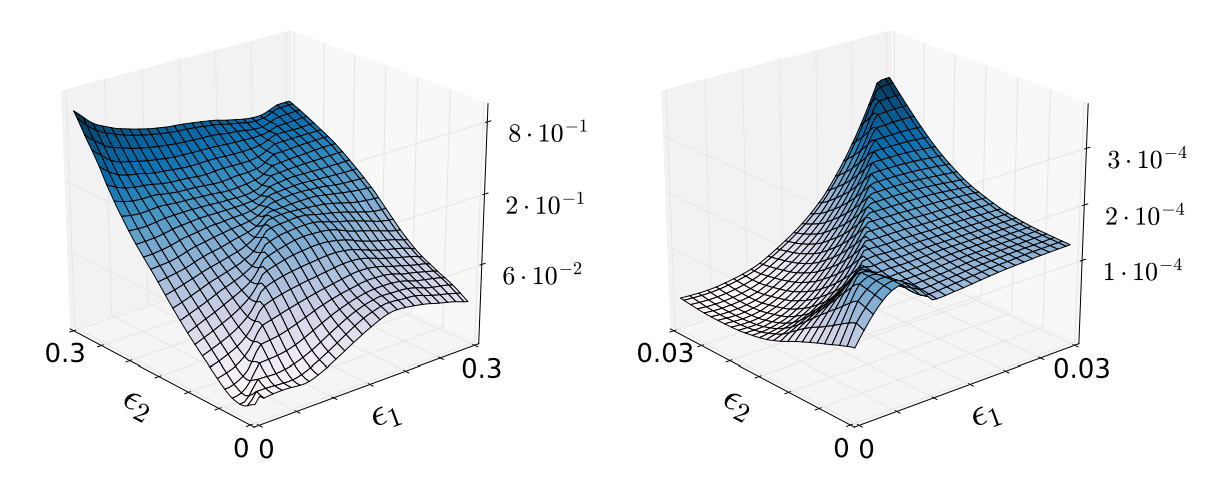
\includegraphics[width=\textwidth]{fig/ob-grad/effect-of-gradient-masking.png}

  \textbf{Note}: $L(\hat{x},y|\theta)$ is still high within $\mathcal{S}$
\end{frame}

\begin{frame}{How to identify them}
  \begin{itemize}
    \item One-step attacks perform better that iterative attacks
    \item Partial random-step attacks perform better
    \item Black-box attacks perform better (see next slide)
    \item Increasing pertubation budget $\epsilon$ doesn't increase success rate pretty much
  \end{itemize}
\end{frame}

\begin{frame}{Why black-box attack can perform better}
  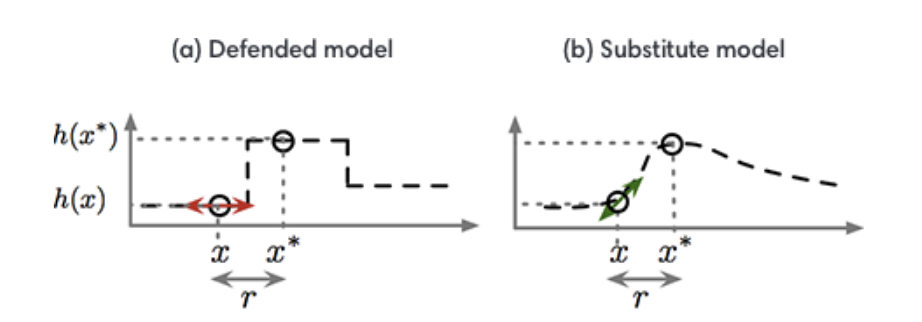
\includegraphics[width=\textwidth]{fig/ob-grad/black-box-attack.png}
\end{frame}

\begin{frame}{Types of Obfuscated Gradients}
  \begin{itemize}
    \item Shattered Gradients 
      \begin{itemize}
        \item non-differentiable operation (\textit{nonexistent})
        \item provide \textit{incorrect} gradient to make adversary stuck in local minima
      \end{itemize}
    \item Random Gradients
        \begin{itemize}
          \item randomize the network
          \item add some random processing to input
        \end{itemize}
      \item Exploding/Vanishing Gradients (?)
  \end{itemize}
\end{frame}

\begin{frame}{Proposed Attack Algorithms}
  \begin{itemize}
    \item Backward Pass Differentiable Approximation (\textit{BPDA})
      \begin{itemize}
        \item Circumvent shattered gradients
        \item $\nabla_xf(g(x))|_{x = \hat{x}} \approx \nabla_xf(x)|_{x = g(\hat{x})}$
      \end{itemize}

    \item Expectation over Transformations (\textit{EOT})
      \begin{itemize}
        \item Circumvent random gradients
        \item $\nabla\mathbb{E}_{t \sim T}f(t(x)) = \mathbb{E}_{t \sim T} \nabla f(t(x))$
        \item In brief, ensemble
      \end{itemize}
  \end{itemize}
\end{frame}

\begin{frame}{Some Thoughts}
  \begin{itemize}
    \item No free lunch, additional cost of
      \begin{itemize}
        \item calculate $g(\cdot)$ many steps
        \item parallel computation cost of ensemble
      \end{itemize}
    \item Succeed attack alg. can be used as defense alg. (remember the minmax objective)
    \item If we make $\epsilon$ larger?
  \end{itemize}
\end{frame}

\subsection{Robustness May Be At Odds With Accuracy}
\begin{frame}{Robustness May Be At Odds With Accuracy}
  
\includegraphics[width=\textwidth]{fig/p2/title.png}
  \center ICLR 2019
\end{frame}

\begin{frame}{Some Highlights}
  \begin{itemize}
    \item Prove trade-off between standard accuracy and robustness \\
      Is adv. training $\in$ Data Augmentation?
    \item Identify robust and non-robust features
    \item Interpretable gradients thru adv. training
  \end{itemize}
\end{frame}

\begin{frame}{Example}
  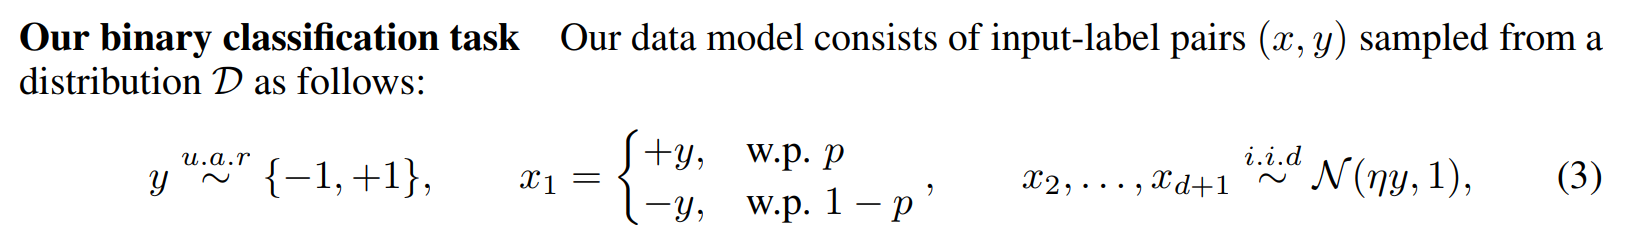
\includegraphics[width=\textwidth]{fig/p2/example.png}
  \begin{itemize}
    \item $x_1$: moderately correlated feature
    \item $x_2 \sim x_{d+1}$: weakly correlated feature, but...
  \end{itemize} 
\end{frame}

\begin{frame}{Accumulation of weakly features}
  Consider the following linear classifier
  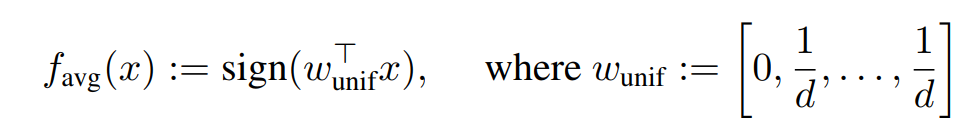
\includegraphics[width=0.8\textwidth]{fig/p2/lc.png}

  if $d$ is large enough
  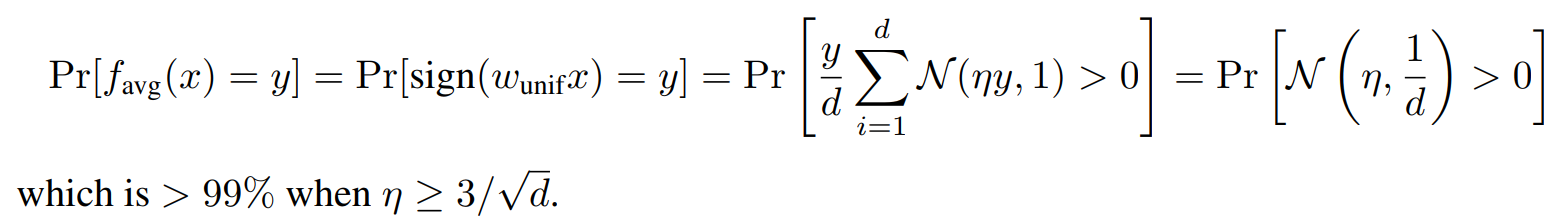
\includegraphics[width=\textwidth]{fig/p2/lc-prob.png}

  \center{The ``meta-feature'' is strongly correlated}
\end{frame}

\begin{frame}{Adversarially robust classification}
  Consider $L_\infty$-bounded adversary with $\epsilon=2\eta$\\
  (You can imagin that two distributions are switched)

  \begin{block}{Theorem: Robustness-accuracy trade-off}
    Any classifier attains at least $1 - \delta$ standard accuracy on $\mathcal{D}$ (the distributions mentioned above) has robust accuracy at most $\frac{p}{1-p}\delta$ against $L_\infty$ bounded adversary with $\epsilon \geq 2\eta$
  \end{block}
\end{frame}

\begin{frame}{Discussion of robust/non-robust features}
  In above case
  \begin{itemize}
    \item $x_1$: robust feature (something invariant)
    \item $x_2 \sim x_{d+1}$: non-robust feature
  \end{itemize}
  \begin{block}{Claim}
    Standard classifier assigns weight to even weakly correlated features, \\but robust classifier doesn't assign any weight beyond a certain thrshold
  \end{block}
\end{frame}

\begin{frame}{Experiments: Binary classifier on MNIST (5 vs 7)}
  \center{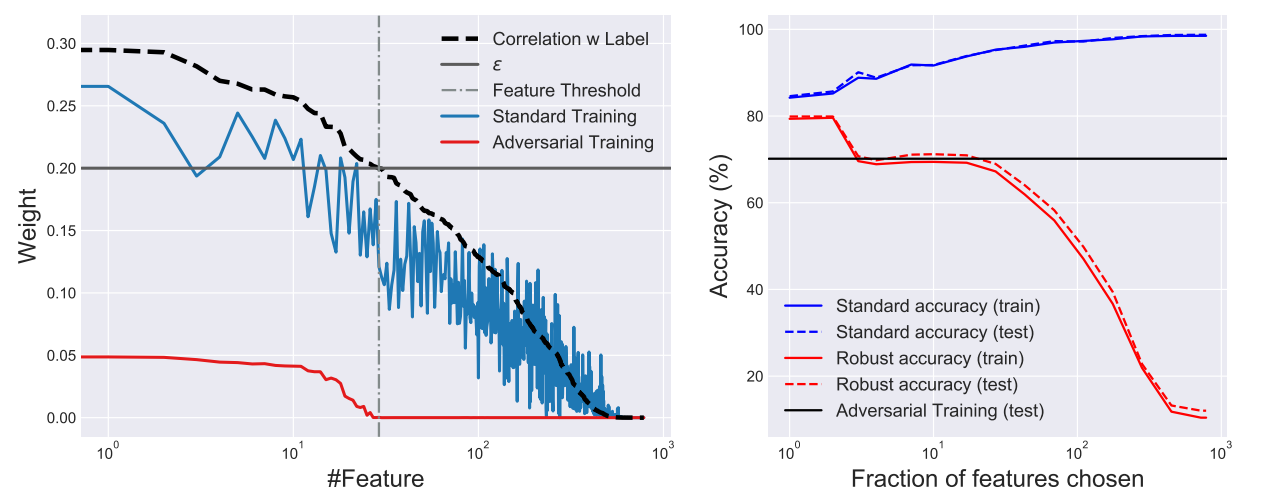
\includegraphics[width=0.8\textwidth]{fig/p2/cu.png}}\\
  Right figure: \\Both accuracy is trained using \textbf{standard} training with subset of features \\
(w/ decreasing relation between label, calculated thru $\mathbb{E}_{(x,y) \sim \mathcal{D}}[yx_i]$)
\end{frame}

\begin{frame}{Interpretable gradients}
  Loss gradients in the input space align well with human eyes
  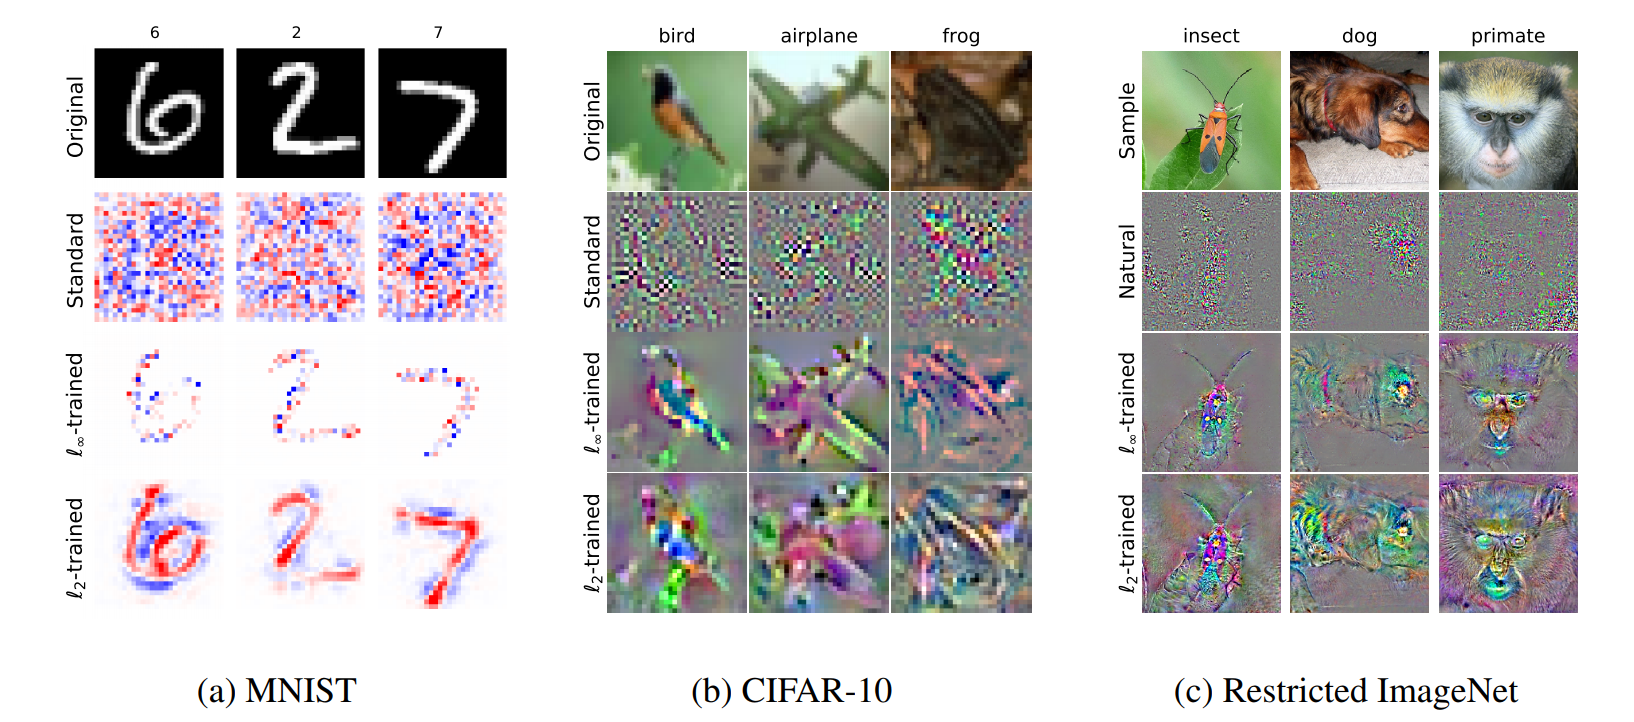
\includegraphics[width=\textwidth]{fig/p2/int-grad.png}
\end{frame}

\begin{frame}{Some Thoughts}
  \begin{itemize}
    \item By encoding appropriate prior into set of pertubations $\mathcal{S}$, adv. training can provide interpretable gradients 
  \end{itemize}
\end{frame}
%\section{Elements}
%\subsection{Fonts}
%\begin{frame}[t]{Fonts}
  %\begin{itemize}
    %\item Regular
    %\item \textit{Italic}
    %\item \textsc{SmallCaps}
    %\item \textbf{Bold}
    %\item \textbf{\textit{Bold Italic}}
    %\item \textbf{\textsc{Bold SmallCaps}}
    %\item \texttt{Monospace}
    %\item \texttt{\textit{Monospace Italic}}
    %\item \texttt{\textbf{Monospace Bold}}
    %\item \texttt{\textbf{\textit{Monospace Bold Italic}}}
  %\end{itemize}
%\end{frame}

%\subsection{Lists}
%\begin{frame}{Lists}
  %\begin{columns}[T,onlytextwidth]
    %\column{0.33\textwidth}
      %Items
      %\begin{itemize}
        %\item Milk \item Eggs \item Potatos
      %\end{itemize}

    %\column{0.33\textwidth}
      %Enumerations
      %\begin{enumerate}
        %\item First, \item Second and \item Last.
      %\end{enumerate}

    %\column{0.33\textwidth}
      %Descriptions
      %\begin{description}
        %\item[PowerPoint] Meeh. \item[Beamer] Yeeeha.
      %\end{description}
  %\end{columns}
%\end{frame}
%\begin{frame}{Animation}
  %\begin{itemize}[<+- | alert@+>]
    %\item \alert<4>{This is\only<4>{ really} important}
    %\item Now this
    %\item And now this
  %\end{itemize}
%\end{frame}

%\subsection{Math}
%\begin{frame}{Math}
  %\begin{equation*}
    %e = \lim_{n\to \infty} \left(1 + \frac{1}{n}\right)^n
  %\end{equation*}
%\end{frame}
\section{MISC}
\begin{frame}
	\begin{center}
    %\weib{\LARGE{謝謝聆聽!}}
    \LARGE{Questions?}
	\end{center}
\end{frame}

\subsection{Interesting papers}
\begin{frame}{Interesting papers about adversarial attack}
  \begin{itemize}
    \item \textit{Towards Deep Learning Models Resistant to Adversarial Attacks} [\href{https://arxiv.org/abs/1706.06083}{link}]
      \begin{itemize}
        \item Survive from attack mentioned above
        \item \textbf{Interesting experiments and insights}
        \item Unreasonable effectiveness of \textbf{Projected} Gradient Descent (PGD)
      \end{itemize}
    \item Universal Pertubations
      \begin{itemize}
        \item \textit{Universal Adversarial Pertubations} [\href{https://arxiv.org/pdf/1610.08401.pdf}{link}], CVPR2017
        \item \textit{Playing The Game Of Universal Adversarial Perturbations} [\href{https://arxiv.org/abs/1809.07802}{link}], rejected by ICLR2019
        \item Quickly reaches high fooling rate, even when the perturbation magnitude $\epsilon$ is small (compared to per-sample pertubation)
      \end{itemize}
  \end{itemize}
\end{frame}

\subsection{Appendix}
\begin{frame}{BPDA}
  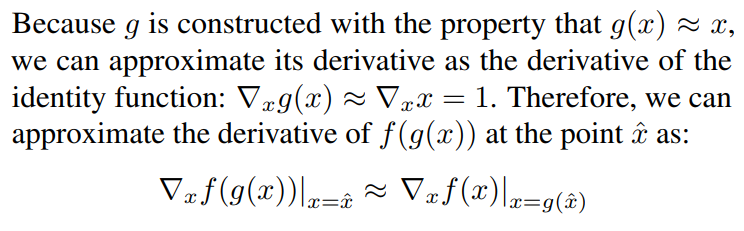
\includegraphics[width=\textwidth]{fig/ob-grad/bpda-fact.png}
\end{frame}

\begin{frame}{Universal Pertubations}
  \center 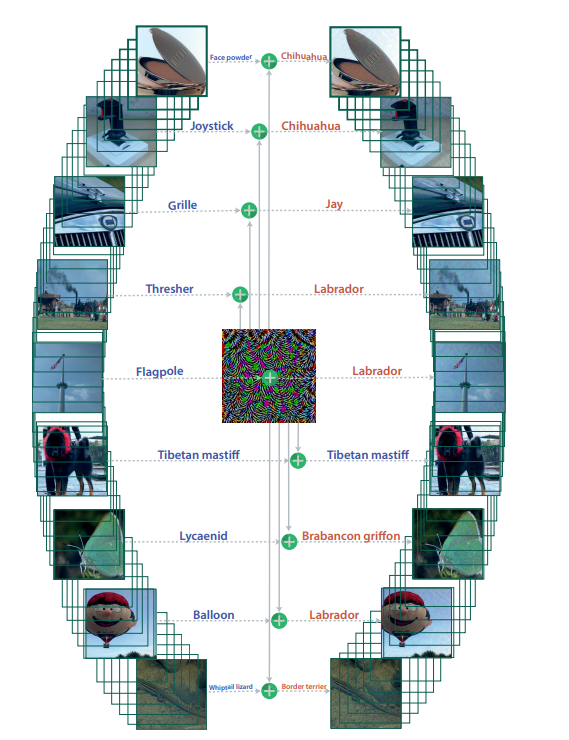
\includegraphics[height=\textheight]{fig/universal-pertubation.png}
\end{frame}
\end{document} 
